\documentclass[twocolumn]{article}
\usepackage[english]{babel}
\usepackage[utf8]{inputenc}
\usepackage{tabto}
\usepackage{dblfloatfix}  
\usepackage{stfloats}
\newcommand\tab[1][1cm]{\hspace*{#1}}
\usepackage[sorting=none]{biblatex} %Imports biblatex package
\addbibresource{dl.bib} %Import the bibliography file

\usepackage[ruled,vlined]{algorithm2e}
\usepackage{tcolorbox}
\usepackage{cuted, lipsum}

\DontPrintSemicolon
\newcommand{\To}{\mbox{\upshape\bfseries to}}


\title{A Deep Reinforcement Learning 
Inspired Local Search for TSP}
\author{Jinchang Fan, Han Wang, Xiaoyu Qiao, Ziyan Lin}
\date{May 2, 2019}

\begin{document}
\maketitle

\begin{strip}
\begin{center}
\begin{abstract}
\centering\begin{minipage}{\dimexpr\paperwidth-10cm}
Many solutions for Traveling Salesman Problem (TSP) have been raised and discussed for a long time, and one of the best approximate solutions is Genetic Algorithm for global search combined with 2-opt for local search. Though accuracy is satisfying, the efficiency of this method is limited by the iterations of 2-opt Heuristic to reach a local optimal. The newly raised Deep Reinforcement Learning also performs well when applied to TSP, but it requires interminable processing time. In this project, half trained Deep Reinforcement Learning Pointer Network is borrowed to provide elitist tour candidates for 2-opt, which would increase the efficiency to find a solution.
\end{minipage}
\end{abstract}
\end{center}
\end{strip}


\section{Introduction}
Traveling Salesman Problem is a famous optimization problem that has been discussed for a long time. The problem asks: given a set of cities and cost of travelling from one to another, what is the best way in terms of cost to visit all cities and come back to the starting point? In contract to its simple description, TSP is found to be an NP-hard problem\cite{gary1979computers}. Considering its popularity and various real-world applications, TSP now performs as a touchstone for different optimizing algorithms. 

So far, algorithms for exact solution of TSP\cite{balinski1964integer}\cite{eilon1974distribution}\cite{laporte1986exact} have been widely developed and discussed respectively, but the solution is still infeasible to reach when the number of cities grows large due to the exponential complexity\cite{helsgaun2000effective}. 

At the same time approximate algorithms\cite{clarke1964scheduling}\cite{gillett1974heuristic} are developed to obtain an acceptable solution in relatively short time, including many bioinspired algorithms\cite{krasnogor2000memetic}\cite{jiao2000novel}\cite{razali2011genetic}. Genetic Algorithm (GA) \cite{whitley1994genetic}  is one of the best algorithms in many combinatorial optimization problems with huge research work thanks to its efficient strategy to reach global optimization, and has been shown to perform quite good on TSP as well\cite{merz1997genetic}. 

The basic procedure of GA on TSP could be described as following: first start with a random initial population and apply local optimizing strategy for each of them, then select instance as ``parents" to generate new off-springs by cross-over breeding. Apply local optimizing strategy again to those off-springs, and partially update population by off-springs after mutation. Repeat generations and population would converge to the global optimization. In the Genetic Algorithm for TSP, local search strategy is critical. A current popular local search method is  2-opt algorithm\cite{lin1973effective}\cite{helsgaun2000effective} with basic idea of performing exchanges of two edges to obtain a shorter tour. This greedy strategy is simple but usually the simplicity is obtained with the danger of failure or inefficiency in finding optimal solutions. The detail of this algorithm is discussed in Section 2.2. 

Reinforcement Learning (RL) in Neural Network\cite{sutton2018reinforcement} is a goal-oriented algorithm that learns to attain some complex goal or maximize value over dimension by discovering which actions yield the most reward. The time consuming work for 2-opt algorithm could be accelerated if the experience from an ideal RL model is learned, and efficiency of the whole Genetic Algorithm is improved consequently. Such improvement would be the main focus of this project. Methodology would be discussed and practice on sample case are performed. The new algorithm is compared with previous work in the evaluation on distance of provided solution and time consumed. 

The rest of this paper is organized as follows. Section 2 introduces a classical algorithm for TSP, namely the combination of 2-opt as local search and Genetic Algorithm for global search. The whole procedure and short coming are discussed in detail.  Section 3 makes a description of the RL-2opt-GA algorithm, and illustrates how it may make an improvement. Section 4 shows how algorithms are realized and compared, including dataset and computation platform.  Section 5 evaluates the result of experiments, and the whole project is summarized in Section 6.

\section{2opt-GA algorithm for TSP}
\subsection{Genetic Algorithm}
Genetic Algorithm is an important tool in solving both constrained and unconstrained optimization problems with inspiration of natural selection. The procedure of  Genetic Algorithm in the context of TSP is illustrated in Figure \ref{fig:ga}. Some important definitions are stated as below.
\begin{itemize}
\setlength\itemsep{0pt}
\setlength\parskip{0pt}
\item Tour: a tour that visits each city exactly one time and returns to the starting point in the end
\item Population: a collection of tours
\item Parents: two tours that could be used to breed children tour
\item Mutation: variation in tours' population, here is a two point swap at random position 
\item Elitism: keep best k tours into the next generation
\end{itemize}

\begin{figure}
\begin{center}
%\begin{tcolorbox}[width=\linewidth*2/3]
\fbox{\begin{minipage}{22em}
\textbf{procedure TSP-GA}
\newline\noindent
\phantom{x}\hspace{0ex}\textbf{begin}
\newline\noindent
\phantom{x}\hspace{3ex}\texttt{initialize population P randomly}
\newline\noindent
\phantom{x}\hspace{3ex}\textbf{foreach} \texttt{tour} $t\in P$ do \textit{2-opt}$(t)$
\newline\noindent
\phantom{x}\hspace{3ex}\textbf{repeat} \textit{\#repeat for generation}
\newline\noindent
\phantom{x}\hspace{6ex} \textbf{repeat} p times: \textit{\#repeat for population}
\newline\noindent
\phantom{x}\hspace{9ex}\texttt{randomly select} $t_{p1},t_{p2}\in P$
\newline\noindent
\phantom{x}\hspace{9ex}$t_{child}:=breed(t_{p1},t_{p2})$
\newline\noindent
\phantom{x}\hspace{9ex}\textit{2-opt}$(t_{child})$
\newline\noindent
\phantom{x}\hspace{9ex}\textbf{With} prob. of 0.01: $Mutation(t_{child})$
\newline\noindent
\phantom{x}\hspace{9ex}\texttt{replace one tour in P by} $t_{child}$;
\newline\noindent
\phantom{x}\hspace{6ex}\textbf{end}
\newline\noindent
\phantom{x}\hspace{3ex}\textbf{until} \texttt{converged};
\newline\noindent
\phantom{x}\hspace{0ex}\textbf{end}
%\end{tcolorbox}
\end{minipage}}
\end{center}
\caption{TSP-GA}
\label{fig:ga}
\end{figure}


\begin{figure}
\begin{center}
%\begin{tcolorbox}[width=\linewidth*2/3]
\fbox{\begin{minipage}{22em}
\textbf{procedure Half-greedy Tour Selection}
\newline\noindent
\phantom{x}\hspace{0ex}\textbf{begin}
\newline\noindent
\phantom{x}\hspace{1ex}\texttt{input maps} \textit{ \#list of cities}
\newline\noindent
\phantom{x}\hspace{1ex}\texttt{N = size(maps)}
\newline\noindent
\phantom{x}\hspace{1ex}\texttt{initialize} $tour = \{\}$
\newline\noindent
\phantom{x}\hspace{1ex}\texttt{length\_of\_tour} = 0
\newline\noindent
\phantom{x}\hspace{1ex}\texttt{randomly select starting city} $c\in maps$
\newline\noindent
\phantom{x}\hspace{1ex}\texttt{tour.append(c)}
\newline\noindent
\phantom{x}\hspace{1ex}\textbf{while} \texttt{length\_of\_tour < N}
\newline\noindent
\phantom{x}\hspace{3ex}\texttt{maps.remove(c)}
\newline\noindent
\phantom{x}\hspace{3ex}\texttt{pool}=\{argsort(dist(c,c\prime)[:3]|$c\prime\in maps$\}
\newline\noindent
\phantom{x}\hspace{3ex}\textit{\#select next city to connect:}
\newline\noindent
\phantom{x}\hspace{3ex}$c_{next} =$\texttt{random.choice(pool,1)}
\newline\noindent
\phantom{x}\hspace{3ex}\texttt{tour.append$(c_{next})$}
\newline\noindent
\phantom{x}\hspace{3ex}\texttt{length\_of\_tour} $+=1$
\newline\noindent
\phantom{x}\hspace{3ex}$c=c_{next}$
\newline\noindent
\phantom{x}\hspace{0ex}\textbf{return} \texttt{tour}
\end{minipage}}
\end{center}
\caption{Half-greedy Tour Selection}
\label{fig:greedy}
\end{figure}


When initializing population in GA, tours with diversity are desired. But connecting points at completely random leads to a lot of work for 2-opt. To balance this problem a half-greedy approach is utilized  as illustrated in Figure \ref{fig:greedy}. A starting city is selected randomly at the beginning. Select next city to connect from the 3 cities with the smallest distances to the starting city. Repeat this process until all cities are visited. Such half-greedy random selection technique will preserve the diversity and utility of tour sets.

In the breeding part of Generic Algorithm, Distance-Preserving Crossover (DPX) has been used. The idea of DPX is to keep child tour having same "distance", in terms of number of common edges, from its two parents. When given two parent tours $t_{p_1}$ and $t_{p_2}$, the initial edges of their child $t_{child}$ tour will be the common edges in $t_{p_1}$ and $t_{p_2}$, and all edges that $t_{p_1}$ and $t_{p_2}$ do not agree with each other are removed. Reconnect components in $t_{child}$ using greedy approach, with restriction that all reconnected edges must not repeat the deleted edges. See pseudo-code in Figure \ref{fig:dpx} for details.
\begin{figure}[h!tb]
\begin{center}
%\begin{tcolorbox}[width=\linewidth*2/3]
\fbox{\begin{minipage}{22em}
\textbf{procedure DPX}
\newline\noindent
\phantom{x}\hspace{0ex}\textbf{begin}
\newline\noindent
\phantom{x}\hspace{3ex}input $t_{p_1},t_{p_2}\in P$
\newline\noindent
\phantom{x}\hspace{3ex}$e_1:=\{edge\in t_{p_1}\}$
\newline\noindent
\phantom{x}\hspace{3ex}$e_2:=\{edge\in t_{p_2}\}$
\newline\noindent
\phantom{x}\hspace{3ex}$\textit{common-edges}:=e_1\cap e_2$
\newline\noindent
\phantom{x}\hspace{3ex}$\textit{destroyed-edges}:=e_1\cup e_2-e_1\cap e_2$
\newline\noindent
\phantom{x}\hspace{3ex}$t_{child} =\{\}$
\newline\noindent
\phantom{x}\hspace{3ex}\textbf{for} $e\in\textit{common-edges}$:
\newline\noindent
\phantom{x}\hspace{6ex}$t_{child} = t_{child}+e$
\newline\noindent
\phantom{x}\hspace{3ex}\textbf{reconnect} $t_{child}$ with greedy approach and 
\newline\noindent
\phantom{x}\hspace{3ex}new edge in $t_{child}$ must not come from \newline\noindent
\phantom{x}\hspace{3ex}\textit{destroyed-edges}
\newline\noindent
\phantom{x}\hspace{0ex}\textbf{end}
%\end{tcolorbox}
\end{minipage}}
%\caption{Figure \ref{box: GADNN}. DPX Procedure}
%\label{box: GADNN}
\end{center}
\caption{DPX Procedure}
\label{fig:dpx}
\end{figure}

Mutation serves as random variant to keep population open to fresh exploring, and happens in low frequency (1\%). To perform mutation on a tour, two cities in tour are randomly swapped to generate variation in the population. 
\subsection{2-opt Algorithm}

The idea of the 2-opt algorithm\cite{helsgaun2000effective} is to obtain a better tour through replacing any two edges by other two ones. Suppose there are n cities the cities salesmen should reach sequentially: $\{c_{1},...,c_{n}\}$. Given the swap position determined as $c_{f}$ and $c_{l}$, the tour is $\{c_{1}$,...$c_{f-1}$,$c_{f}$,$c_{f+1}$,...,$c_{l-1}$,$c_{l}$,$c_{l+1}$,...,$c_{n}\}$, then edge ($c_{f}$, $c_{f-1}$) and ($c_{l}$, $c_{l+1}$) are replaced by ($c_{l}$,$c_{f-1}$) and ($c_{f}$, $c_{l+1}$). The new tour turns to be  $\{c_{1}$,...,$c_{f-1}$,$c_{l}$,$c_{last-1}$,...,$c_{f+1}$,$c_{f}$,$c_{l+1}$...,$c_{n}\}$. The 2-opt algorithm is shown in detail in Figure \ref{fig:2opt}.
\begin{figure}[h!tb]
\begin{center}
%\begin{tcolorbox}[width=\linewidth*2/3]
\fbox{\begin{minipage}{22em}
\textbf{2-opt Algorithm}
\newline\noindent
\phantom{x}\hspace{0ex}\textbf{begin}
\newline\noindent
\phantom{x}\hspace{0ex}{Initialize tour }$t${ and best-distance.}
\newline\noindent
\phantom{x}\hspace{0ex}{Let} \texttt{count} $= 0$.
\newline\noindent
\phantom{x}\hspace{0ex}\textbf{while} (the tour is still improving):
\newline\noindent
\phantom{x}\hspace{3ex}\textbf{for} $c_{first}${ in range(1,(len(tour)-2)):}
\newline\noindent
\phantom{x}\hspace{5ex}\textbf{for} $c_{last}${ in range(}$c_{first}${+1,len(tour):}
\newline\noindent
\phantom{x}\hspace{7ex}{Del (}$c_{first}${, }$c_{first-1}${) and (}$c_{last}${, }$c_{last+1}${)}
\newline\noindent
\phantom{x}\hspace{7ex}{Build (}$c_{last}${, }$c_{first-1}${) and (}$c_{first}${, }$c_{last+1}${)}
\newline\noindent
\phantom{x}\hspace{7ex}Calculate new-distance
\newline\noindent
\phantom{x}\hspace{7ex}\textbf{if} {new-distance }$<${best-distance:}
\newline\noindent
\phantom{x}\hspace{9ex}\textbf{Update} tour and best-distance
\newline\noindent
\phantom{x}\hspace{9ex}{count }$+=1$
\newline\noindent
\phantom{x}\hspace{0ex}
\textbf{end}
\end{minipage}}
\end{center}
\caption{2-opt Algorithm}
\label{fig:2opt}
\end{figure}

In this procedure each pair of cities should be checked with a total number of $O(n^2)$ times. Effort can be saved if somehow narrowing down the size of potential cities to be tried instead of trying all probable exchanges. Fortunately, some idea from Reinforcement Learning could help with this narrowing, plus with improvement coming from efficiency in moving trace. It would be discussed in detail in next section.

\section{RL-2opt-GA}

\begin{figure*}[h!t]
 \centering
\includegraphics[width = 15cm]{PN_attention.jpg}
\caption{Pointer Network with Bahdanau Attention\cite{bahdanau2016end}}
\label{fig:attention}
\end{figure*}

In terms of TSP, swap based local search wants to minimize the distance of tour by making greedy improvement each step. In this non-convex situation it may move in a zigzag way with relatively slow speed to reach the local optimal. Instead of greedy strategy, Reinforcement Learning is trained to make a decision in prospect of future reward. In this project a learning result from Reinforcement Learning, namely the transition operator based on probabilities is applied to 2-opt step, as each swap operation in 2-opt process are formed according to those probabilities. Besides narrowing down the pool to be checked out, guide from Reinforcement Learning prefers long term reward and will lead a way reaching local optimal in less steps. Such a combination will provide a more efficient and effective way for tour selection and generation.

\subsection{Pointer Network and Reinforcement Learning}
As a modification of Recurrent Neural Network\cite{jaeger2002tutorial}, Pointer Network\cite{vinyals2015pointer} uses attention as a pointer to give anoutput by selecting a member from the input sequence. The structure of Pointer Network (PN) utilizing Bahdanau Attention is shown in Figure \ref{fig:attention}.

The parameters of a Pointer Network can be optimized using the well-known REINFORCE algorithm\cite{bello2016neural}. See Figure \ref{fig:rl} for detail.

Although an independent use of Reinforcement Learning could provide a solution by itself, it requires a large scale of data and time for calculations. A new procedure RL-2opt-GA, as proposed in below section, is a combined algorithm of Reinforcement Learning, 2-opt and Generic Algorithm. In this algorithm PN is half-trained based on relatively small data load to save effort, while it is still able to generate a well-performing optimal tour.

\begin{figure}[h!tb]
\begin{center}
%\begin{tcolorbox}[width=\linewidth*2/3]
\fbox{\begin{minipage}{22em}
\textbf{REINFORCE Algorithm}
\newline\noindent
\phantom{x}\hspace{0ex}\texttt{training set = T} 
\newline\noindent
\phantom{x}\hspace{0ex}\texttt{batch size = B}
\newline\noindent
\phantom{x}\hspace{0ex}\textbf{repeat}
\newline\noindent
\phantom{x}\hspace{1ex} $s_{i} \sim sample(T)$ for $i \in\{1, \ldots, B\}$
\newline\noindent
\phantom{x}\hspace{1ex} $\pi_{i} \sim sample\left(p_{\theta}\left( \cdot| s_{i}\right)\right)$for $i \in\{1, \ldots, B\}$
\newline\noindent
\phantom{x}\hspace{1ex} $g_{\theta} \leftarrow \frac{1}{B} \sum_{i=1}^{B}\left(L\left(\pi_{i} | s_{i}\right)-b_{i}\right) \nabla_{\theta} \log p_{\theta}\left(\pi_{i} | s_{i}\right)$
\newline\noindent
\phantom{x}\hspace{1ex} $\theta \leftarrow \operatorname{ADAM}\left(\theta, g_{\theta}\right)$
\newline\noindent
\phantom{x}\hspace{1ex} \textbf{until convergence}
\newline\noindent
\phantom{x}\hspace{0ex}\textbf{return }$p_{\theta}$
%\end{tcolorbox}
\end{minipage}}
\end{center}
\caption{REINFORCE Algorithm (Source: \cite{bello2016neural})}
\label{fig:rl}
\end{figure}


After optimizing the Pointer Network with REINFORCE algorithm, the $n\times n$ matrix of probabilities D will be returned. Notice that in PN the probabilities come out as a sequence corresponding to actions at each step, but the collected $D[i,j]$ just represents the probability of connecting city $j$ as the next when city $i$ has just reached without considering any other edges. In other word, given different starting point, first step of each sequence is collected.


\subsection{A Reinforcement Learning Inspired Local Search}

As the decision matrix D comes from a half-trained Pointer Network, no doubt that its suggestion is far away from the best. But for a 2opt-GA model, it is enough to make some improvement, as all suggestions are tested and the useful one with good output would be found. This good "character" learned form D would be saved and breed off to the whole population, and eventually shows in optimal tour.  In terms of efficiency, 2-opt performs a work with complexity $O(n^2)$ as mentioned previously. With the help of decision matrix D, for each city $i$, only k cities with largest probabilities in D[i,:] need to be checked, which requires $O(n)$ times. The 2-opt algorithm based on decision matrix is shown in detail in Figure \ref{fig:2opt2}.

\begin{figure}[h!tb]
\begin{center}
%\begin{tcolorbox}[width=\linewidth*2/3]
\fbox{\begin{minipage}{22em}
\textbf{2-opt Algorithm Based on Decision Matrix}
\newline\noindent
\phantom{x}\hspace{0ex}\textbf{begin}
\newline\noindent
\phantom{x}\hspace{0ex}Initialize tour $t$ and \textit{best-distance}
\newline\noindent
\phantom{x}\hspace{0ex}Input decision matrix $D$
\newline\noindent
\phantom{x}\hspace{0ex}Let count $= 0$
\newline\noindent
\phantom{x}\hspace{0ex}\textbf{while} {(the tour is still improving)}:
\newline\noindent
\phantom{x}\hspace{3ex}\textbf{for }$c_{first}${ in range(1,(len(tour)-2)):}
\newline\noindent
\phantom{x}\hspace{5ex}$D_{c_{first}}=\{d_1,...,d_K\}$
\newline\noindent
\phantom{x}\hspace{5ex}$C=${ the corresponding cities}
\newline\noindent
\phantom{x}\hspace{5ex}\textbf{for} $c_{last}${ in }$C${:}
\newline\noindent
\phantom{x}\hspace{7ex}{Del (}$c_{first}${, }$c_{first-1}${) and (}$c_{last}${, }$c_{last+1}${)}
\newline\noindent
\phantom{x}\hspace{7ex}{Build (}$c_{last}${, }$c_{first-1}${) and (}$c_{first}${, }$c_{last+1}${)}
\newline\noindent
\phantom{x}\hspace{7ex}Calculate new-distance
\newline\noindent
\phantom{x}\hspace{7ex}\textbf{if} \textit{new-distance }$<$\textit{best-distance:}
\newline\noindent
\phantom{x}\hspace{9ex}\textbf{Update} \textit{tour} and \textit{best-distance}
\newline\noindent
\phantom{x}\hspace{9ex}{count }$+=1$
\newline\noindent
\phantom{x}\hspace{1ex}
\textbf{end}
%\end{tcolorbox}
\end{minipage}}
%\caption{2-opt Algorithm based on decision matrix}
%\label{box: LK2}
\end{center}
\caption{2-opt Algorithm with Decision Matrix}
\label{fig:2opt2}
\end{figure}

\begin{figure}[H]
%\begin{tcolorbox}[width=\linewidth*2/3]
\fbox{\begin{minipage}{22em}
\textbf{procedure RL-optimized PN}
\newline\noindent
\phantom{x}\hspace{0ex}\#Begin RL
\newline\noindent
\phantom{x}\hspace{0ex}\textbf{Initial} maps = \texttt{cities}(50)
\newline\noindent
\phantom{x}\hspace{0ex}\textbf{Initial} tours = \texttt{train\_tours}(10000)
\newline\noindent
\phantom{x}\hspace{0ex}\textbf{begin} \texttt{forward}:
\newline\noindent
\phantom{x}\hspace{3ex}\texttt{probs = PN(maps, attention)}
\newline\noindent
\phantom{x}\hspace{3ex}\texttt{decision = Route(probs, start\_city)}
\newline\noindent
\phantom{x}\hspace{3ex}\texttt{eval = evaluation(decision)}
\newline\noindent
\phantom{x}\hspace{0ex}\#Gradient Descent optimization for PN
\newline\noindent
\phantom{x}\hspace{0ex} \texttt{PN\_opt = RL(eval)}
\newline\noindent
\phantom{x}\hspace{0ex} \texttt{D = PN\_opt(maps)}
\newline\noindent
\phantom{x}\hspace{0ex}\textbf{return} \texttt{decision matrix D}
\end{minipage}}

\label{fig:rlPN}\caption{RL-optimized PN}
\end{figure}
\begin{figure}[H]
%\begin{tcolorbox}[width=\linewidth*2/3]
\fbox{\begin{minipage}{22em}
%\textbf{procedure RL-2opt-GA}
\newline\noindent
\phantom{x}\hspace{0ex}\textbf{begin GA}
\newline\noindent
\phantom{x}\hspace{0ex}\texttt{initialize population P}
\newline\noindent
\phantom{x}\hspace{0ex}\textbf{foreach} \texttt{tour} $t\in P$ do $LocalSearch(t)$
\newline\noindent
\phantom{x}\hspace{3ex}\textbf{repeat} \textit{\#repeat for generation}
\newline\noindent
\phantom{x}\hspace{6ex} \textbf{repeat} p times: \textit{\#repeat for population}
\newline\noindent
\phantom{x}\hspace{9ex}\texttt{randomly select} $t_{p1},t_{p2}\in P$
\newline\noindent
\phantom{x}\hspace{9ex}$t_{c}:=breed_{DPX}(t_{p1},t_{p2})$
\newline\noindent
\phantom{x}\hspace{9ex}\textit{2-opt}$(t_c,D)$
\newline\noindent
\phantom{x}\hspace{9ex}$Mutation(t_c)$
\newline\noindent
\phantom{x}\hspace{9ex}\texttt{replace one tour in P by} $t_c$
\newline\noindent
\phantom{x}\hspace{6ex}\textbf{end}
\newline\noindent
\phantom{x}\hspace{3ex}\textbf{until} \texttt{converged}
\newline\noindent
\phantom{x}\hspace{0ex}\textbf{end}
%\end{tcolorbox}
\end{minipage}}
\caption{RL-2opt-PN}
\label{fig:rl2optpn}
\end{figure}

\section{Datasets and Experiments}
Python and PyTorch is used to realize computing work in this project, on the cloud server \url{www.sciserver.org}. The dataset, instances of 50 cities on a map,  are randomly generated by sampling uniform distributed point from the range $[0,1]*[0,1]$, and cost between cities is measured by Euclidean distance.


To compare the classical 2opt-GA algorithm and RL-2opt-GA with decision matrix, distances of optimal solution and running time are reported for 30 randomly generated maps. Both algorithm runs genetic evolution with total population of 30, maximum 30 iterations.

\begin{table*}[tbph]
  \centering
\begin{tabular}{l|l|llll}
                  & \multicolumn{1}{c|}{\multirow{Time (sd)}} & \multicolumn{4}{c}{Distance}\\ \cline{3-6} 
                  & \multicolumn{1}{c|}{}                      & \multicolumn{1}{l|}{Iteration 0} & \multicolumn{1}{l|}{Iteration 10} & \multicolumn{1}{l|}{Iteration 20} & Iteration 30 \\ \hline
RL-2opt-GA with D & 499.9 ( 9.195)                            & \multicolumn{1}{l|}{5.78444}     & \multicolumn{1}{l|}{5.72206}      & \multicolumn{1}{l|}{5.71061}      & 5.70458      \\
RL-2opt-GA        & 579.1 (10.962)                           & \multicolumn{1}{l|}{5.78523}     & \multicolumn{1}{l|}{5.71853}      & \multicolumn{1}{l|}{5.70684}      & 5.70307     
\end{tabular}
\caption{Result Comparison}
  \label{tab:1}
\end{table*}

\section{Evaluation}
Among these optimal solutions, distance of the tour will be viewed as main standard to evaluate results. The shortest distance will be treated as standard level, and all other solutions will be divided by this standard level to measure how much worse they are compared with standard level. Average will be another important measurement to evaluate outputs. Instead of arithmetic mean, geometric mean is measured as it is more stable when affected by extreme values. All $n$ optimal solutions will be multiplied together and then take $n^{th}$ root on its product.

Table \ref{tab:1} shows the comparing of classical 2opt-GA and RL-2opt-GA, in terms of running time in arithmetic mean  and optimal solutions in geometric mean during iteration. Update of each iteration in terms of scaled distance of tour is shown in Figure \ref{fig:result}. The distance of optimal solution from two algorithm is almost the same, and RL-2opt-GA finishes the task in shorter time, which indicates that information from decision matrix do provide instructions for long term improvement, and move ahead more directly to a local optimal.

\begin{figure}[tbph]
    \centering
    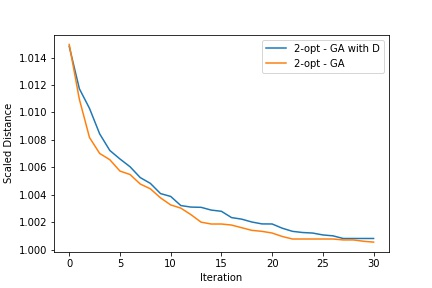
\includegraphics[width = 0.5\textwidth]{result.jpg}
    \caption{cost of optimal solutions during iteration}
    \label{fig:result}
\end{figure}

\section{Summary}
The implement of Deep Reinforcement Learning provides information about decision matrix to improve solutions from 2-opt algorithm. Thanks to prospective knowledge contained in decision matrix, the outputs obtained by modified algorithm are better than original 2-opt algorithm. 

There are still some improving space for this project. Firstly, no information of the tour before 2-opt is involved in decision matrix currently. If such information could be taken into consideration, local search may be more efficient. Secondly, Deep Reinforcement Learning is trained on 10,000 graphs, which is far away from well-educated. Though quick training is desired for efficiency's sake, more rigorous tuning should be performed to find out the optimal training size. Thirdly, the size of cities is too small to tell a difference between algorithms, even no significant improvement from a simple local optimal to global optimal (solution of a pure local search is only 1.4\% worse than solution after global search). Theoretically, with the increasing of city size, the problem becomes more and more complicated and greedy algorithm would be stuck. Due to the limitation of computation resource, experiment on large scale dataset is not performed here.
%yeah yeah yeah 
\newpage
\printbibliography



\end{document}
